\chapter{Oscillations and Waves}

\textbf{Periodic Motion} is a motion that regularly returns a certain position after fixed time.
\textbf{Simple Harmonic Motion} is a special kind of periodic motion where the magnitude of the 
net force acting on an object is proportional to the position of said object and its direction
opposite of the displacement of said object relative to its equilibrium position.

\section{Motion of an Object Attached to a Spring}

Consider the following system.

\begin{center}
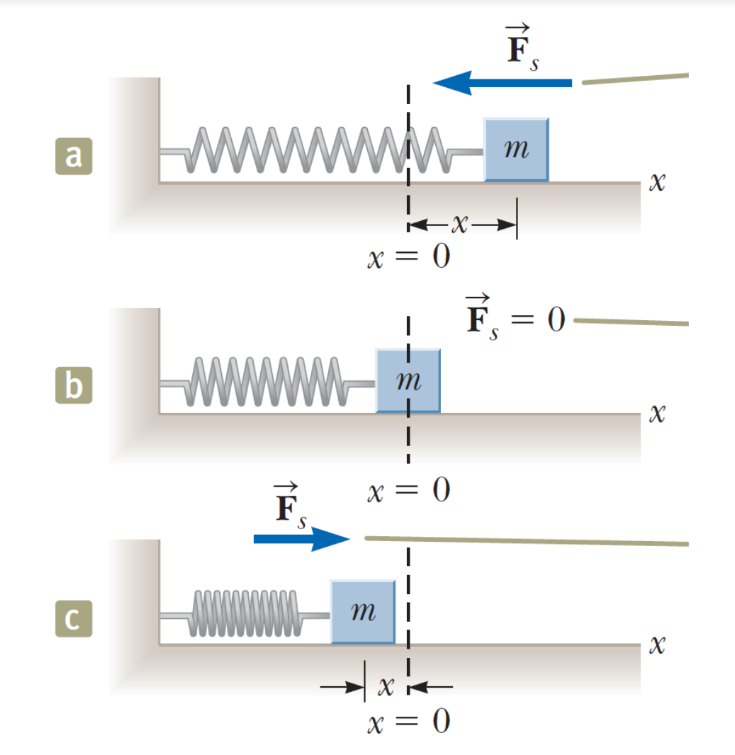
\includegraphics[scale=0.5]{oaw/spring01.png}\label{fig15.1}
\end{center}

When the spring is neither stretched or compressed, the block is at the \textbf{equilibirum position},
denoting as $x = 0$. When force is applied, the position of the block will move back and forth in an 
oscillating motion. We can model this using Hooke's law.

\begin{equation}\label{15.1}
    F_s = -kx
\end{equation} 

Here, we call $F_s$ the \textbf{restoring force} as it is always directed towards the equilibrium position.
Thus, it will always be opposite of the displacement of the block. Since there is some net force
acting on the object, even when released, we can apply Newton's second law of motion onto~\eqref{15.1}
to obtain

\begin{equation*}
    \sum F_x = ma_x \rightarrow -kx = ma_x
\end{equation*}

\begin{equation}\label{15.2}
    a_x = - \frac{k}{m}x
\end{equation}

This shows that the force applied on the object is proportional to $x$ and direction is opposite 
of the displacement. This is an example of a simple harmonic motion.

An example of how an object moves $-$ given the object starts at displacement $x=A$ and $x=0$ is the
equilibrium position:
\begin{itemize}
    \item Once released from rest, initial acceleration $a_i = -kA/m$ and speed is 0
    \item Once block is at $x=0$, acceleration is also zero and speed is at maximum
    \item Passing $x=0$, it moves with positive acceleration until $x=-A$, $a = +kA/m$, and speed is 0
    \item Moves back and passes $x=0$ again with maximum speed
\end{itemize}

In conclusion, the object oscillates between $x \in [-A, A]$. Note that we are consider this system
in the absence of friction. However, real-world systems are not frictionless, so please do keep that in mind.

\section{Analysis Model: Particle in Simple Harmonic Motion}

Recall equation from~\eqref{15.2}, we can turn $a$ into $d^2x / dt^2$ since accerelation is just
the second derivative of displacement and express it as
\begin{equation}\label{15.3}
    \frac{d^2x}{dt^2} = -\frac{k}{m}x
\end{equation}

We can then express $k/m$ as $\omega^2$ then rewrite~\eqref{15.3} as 
\begin{equation}\label{15.5}
    \frac{d^2x}{dt^2} = - \omega^2 x
\end{equation}

We now arrive at a differential equation that we need to solve. In essence, we are trying to 
find a function $x$ whose second-order derivative is the same as the original with a negative sign
and multiplied by $\omega^2$.
We have a few choices: polynomic with negative power, exponential, logarithmic, and trigonometric
functions. Our choice? \textit{Trigonometric functions}, specifically $\sin$ and $\cos$. Finally,
we have found a suitable function $x$.
\begin{equation}\label{15.6}
    x(t) = A\sin(\omega t + \phi)
\end{equation} 
where $A$, $\omega$, and $\phi$ are constant parameters of the motion. Then, we can plot $x$ as
a function of $t$. These parameters (and some more) will then represent the following:
\begin{itemize}
    \item $A$ represents the \textbf{amplitude} $-$ the maximum value of position such that $|x|\leq A$
    \item $\omega$ represents the \textbf{angular frequency} $-$ measure of how rapidly the oscillations
        are occurring, where \begin{equation}\label{15.9}
            \omega = \sqrt{\frac{k}{m}}
        \end{equation}
    \item $\phi$ represents the \textbf{phase constant} or \textbf{initial phase angle} $-$
        determined by the position and velocity position and velocity of object at $t=0$, where
        if $x=A$ at $t=0$, $\phi = 0$
\end{itemize}

Another quantity to know is $(\omega t + \phi)$ or the \textbf{phase} of the motion.
Notice that the value of $x(t)$ has the same value when the $\omega t$ increases by $2\pi$ radians.

Now, we will also introduce another value $T$ representing the \textbf{period} which refers to 
the time interval for an object to go through a full cycle of motion. This essentially means that 
the speed and position of the object at time $t$ and $t+T$ will be the same. This can be further
summarized $-$ using the property of phase $-$ down to 
\[ \left[\omega(t + T) + \phi\right] - (\omega t +\phi) = 2\pi \]
since when the phase is added by $2\pi$, the $x(t)$ reverts to its original value.

Simplifying the above equation gives us
\begin{equation}\label{15.10}
    T = \frac{2\pi}{\omega}
\end{equation}

One more quantity we should know is the \textbf{frequency} $f$, the inverse of the period.
Since the period is the time interval per oscillation, the frequency is oscillations per time interval.
This can be modeled under
\begin{equation}\label{15.11}
    f = \frac{1}{T} = \frac{\omega}{2\pi}
\end{equation}
and its units are cycles per second or \textit{hertz} (Hz). Rearranging the above equation yields
\begin{equation}\label{15.12}
    \omega = 2\pi f = \frac{2\pi}{T}
\end{equation}

If we converted $\omega$ back to its original value of $\sqrt{k/m}$, we will notice that $T$ and $f$
depend solely on the mass of the object and the force constant of the spring.

Additionally, since $x(t) = A\sin(\omega t + \phi)$ represents the position of the object, we can
find the velocity and acceleration squared of the object under S.H.M. using
\begin{eqnarray}
    v = \frac{dx}{dt} = \omega A\cos(\omega t + \phi)\label{15.15}\\
    a = \frac{d^2x}{dt^2} = -\omega^2 A\sin(\omega t + \phi)\label{15.16}
\end{eqnarray}

Notice from both equations that since $\cos$ and $\sin$ both have range of $[-1, 1]$, the range of 
the velocity and acceleration are as following
\begin{eqnarray}
    v_{\max} = \omega A\\
    a_{\max} = \omega^2 A
\end{eqnarray}

\section{Energy of Simple Harmonic Oscillator}

Once we have analyzed a S.H.M. with its forces, we now analyze it with its energy. Consider the 
same system from~\ref{fig15.1}. Let us make a few assumptions: that our spring has no mass and the 
surface is frictionless.

Recall equation~\eqref{15.15}, we can use it to express the kinetic energy of the block as 
\begin{equation}\label{15.19}
    K = \frac{1}{2}mv^2 = \frac{1}{2}m\left(\omega^2 A^2 \cos^2(\omega t + \phi)\right)
\end{equation}
We refer to this as the \textit{kinetic energy of a simple harmonic oscillator}.

Then, we can use equation~\eqref{15.16} for the elastic potential energy from the spring
\begin{equation}\label{15.20}
    U = \frac{1}{2}kx^2 = \frac{1}{2}k\left(A^2 \sin^2(\omega t + \phi)\right)
\end{equation}
We refer to this as the \textit{potential energy of a simple harmonic oscillator}.

\begin{center}\label{fig15.9}
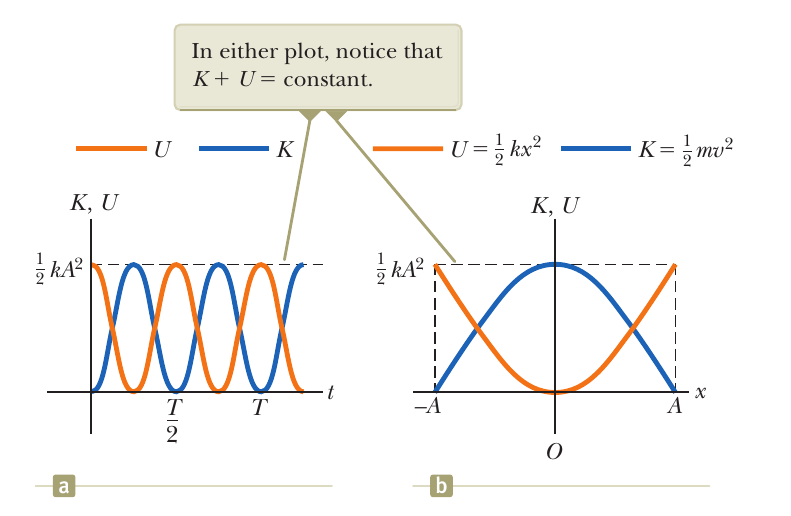
\includegraphics[scale=0.5]{images/oaw/fig15_9.png}
\end{center}
Once plotted, notice that $K$ and $U$ are always positive or zero. We can then express the total
mechanical energy of the system as 
\begin{equation}\label{fullE}
    E = K + U = \frac{1}{2}kA^2\left[ \cos^2(\omega t + \phi) + \sin^2(\omega t + \phi) \right]
\end{equation}

Using trigonometric identity, we can simplify $E$ down to 
\begin{equation}\label{15.21}
    E = \frac{1}{2}kA^2
\end{equation}

This shows that $E$ is a constant of the motion and proportional to the square of the amplitude.
Notice that at the end of the day, it is simply a conversion between the the kinetic and potential
energy. Thus, their sum will always be equal to $(1/2)kA^2$.

\section{Pendulum}

Consider the following \textit{simple pendulum}
\begin{center}
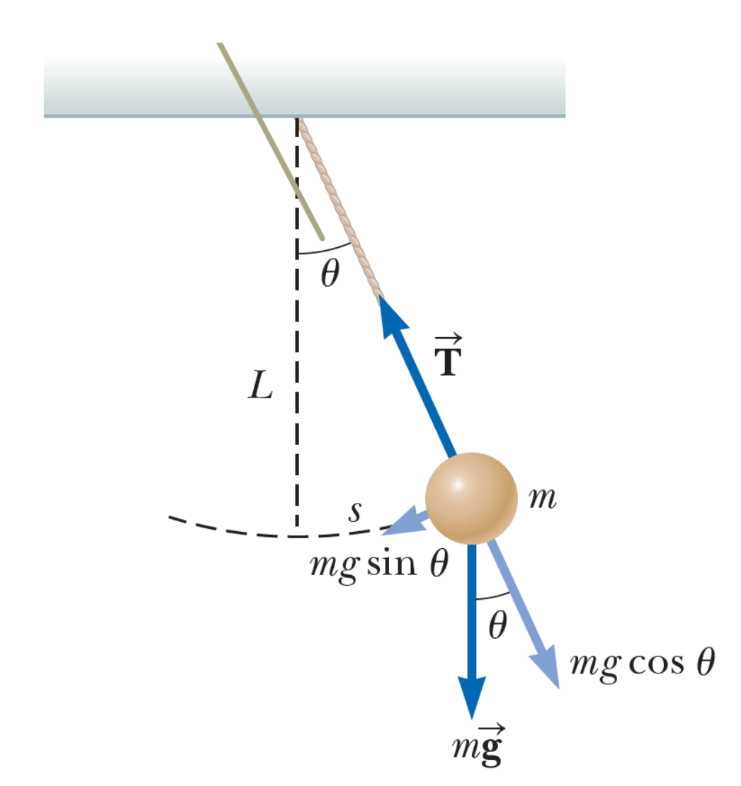
\includegraphics[scale=0.6]{images/oaw/pendulum01.png}
\end{center}
It consists of a bob with mass $m$ suspended by a light string of length $L$. Now, let us
show that given that $\theta$ is small, the motion is very close to being simple harmonic.

The external forces acting upon the bob are the gravitational force $m\vec{g}$ and the tension
$\vec{T}$. Notice that the tangential component of the gravitational force $m\vec{g}\sin\theta$
always acts towards $\theta = 0$, which is opposite of the displacement relative to equilibrium.
Thus, we can denote the tangential component as the \textit{restoring force}. Using Newton's 
second law, we obtain
\[ F_t = ma_t \rightarrow -mg\sin\theta = m\frac{d^2s}{dt^2} \] 
where $s$ denotes the bob's position along the arc. Since $s = L\theta$, this reduces to
\[ \frac{d^2\theta}{dt^2} = - \frac{g}{L}\sin\theta \]

This is where we need to face the harshness of reality. We cannot solve this equation, not without
a computer. However, we can use some approximation tricks to help us. If the angle of swing $\theta$ 
is small ($< 10^\circ$), $\sin\theta \approx \theta$ in radians. Thus, we obtain
\begin{equation}
    \frac{d^2\theta}{dt^2} \approx -\frac{g}{L}\theta
\end{equation}

Now, we cn conclude that the motion of pendulums with small amplitudes can be modelled as simple 
harmonic motion. Therefore, the (approximate) solution to this equation of motion is
\begin{equation}
    \theta(t) = A\sin(\omega t + \phi), \omega = \sqrt{\frac{g}{L}}
\end{equation}
where $A$ is the maximum angular position or $\theta_{\max}$.

From the above equations, we can also derive that the period of this motion is
\begin{equation}
    T = \frac{2\pi}{\omega} = 2\pi\sqrt{\frac{L}{g}}
\end{equation}

In this case, mass does not even matter to the oscillation. The only things that matter are the 
gravitational accerelation ($g$) and the length of the string attached to your pendulum ($L$).
Interestingly, this was how people made clocks back in the day.

\subsection{Physical Pendulum}

Consider the following object pivoted at point $O$ at distance $d$ from the center of mas $CM$.
The gravitational force provides torque with magnitude $mgd\sin\theta$ as shown in the diagram below.

\begin{center}
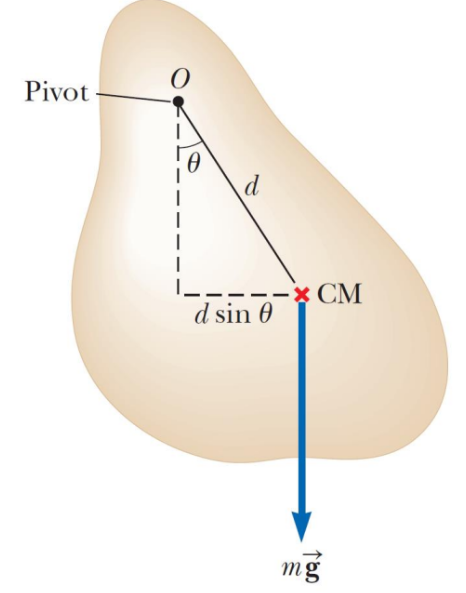
\includegraphics[scale=0.5]{images/oaw/rotation01.png}
\end{center}

We then apply the rotational form of Newton's second law $\vec{\tau} = I\vec{\alpha}$ where $I$ is
the moment of inertia, resulting in 
\[ -mgd \sin\theta = I\frac{d^2\theta}{dt^2} \]
Similar to the simple pendulum, the gravitational force is acting as the restoring force.
Also note that the reason that we use $mgd\sin\theta$ instead of $mgd$ alone is because $\tau$ is
calculated using the perpendicular distance to the force acting on it (gravitational force in this
case).

Assuming that $\theta$ is small, we can use still use the approximation of $\sin$ which reduces the 
equation of motion to 
\begin{equation}\label{15.27}
    \frac{d^2\theta}{dt^2} = -\left(\frac{mgd}{I}\right)\theta = -\omega^2\theta
\end{equation}

Solving~\eqref{15.27} yields 
\begin{equation}
    \theta = A\sin(\omega t + \phi), \omega = \sqrt{\frac{mgd}{I}}
\end{equation}
where $A$ is the maximum angular position.

The period can also be computed with 
\begin{equation}\label{15.28}
    T = \frac{2\pi}{\omega} = 2\pi\sqrt{\frac{I}{mgd}}
\end{equation}
This can also be used to find the moment of inertia of a flat, rigid object, given that the location 
of CM is and $d$ is known.

\section{Damped Oscillations}

So far, we have only analyzed ideal systems where the oscillations will continue indefinitely.
However, that is not realistic as friction and air resistance exist in real systems. Consequently,
$E$ of the system decreases over time and the motion is considered \textbf{damped}. This done through 
the conversion of mechanical energy into internal energy.

The force that decreases the total mechanical energy of the system is referred as the \textbf{retarding
force}. A common type is when the force is proportional to the speed and acts in the opposite direction 
of the velocity of the object. Letting $\vec{R} = -b\vec{v}$ be the retarding force where $b$ is a
constant called the \textbf{damping coefficient} and $-kx$ being the restoring force, we can express 
Newton's second law as \[ \sum F_x = -kx -bv_x = ma_x \] 
then rearranged into
\begin{equation}\label{15.31}
    -kx - b\frac{dx}{dt} = m\frac{d^2x}{dt^2}
\end{equation}

When $b$ is small, the solution to~\eqref{15.31} is
\begin{equation}
    x = Ae^{-(b/2m)t}\cos(\omega t + \phi)
\end{equation}
where the angular frequency of oscillation is 
\begin{equation}
    \omega = \sqrt{\frac{k}{m} - {\left(\frac{b}{2m}\right)}^2}
\end{equation}
Here, $\sqrt{k/m}$ represents the \textit{natural frequency} of the system, which is essentially the 
undamped oscillator.

\begin{center}
    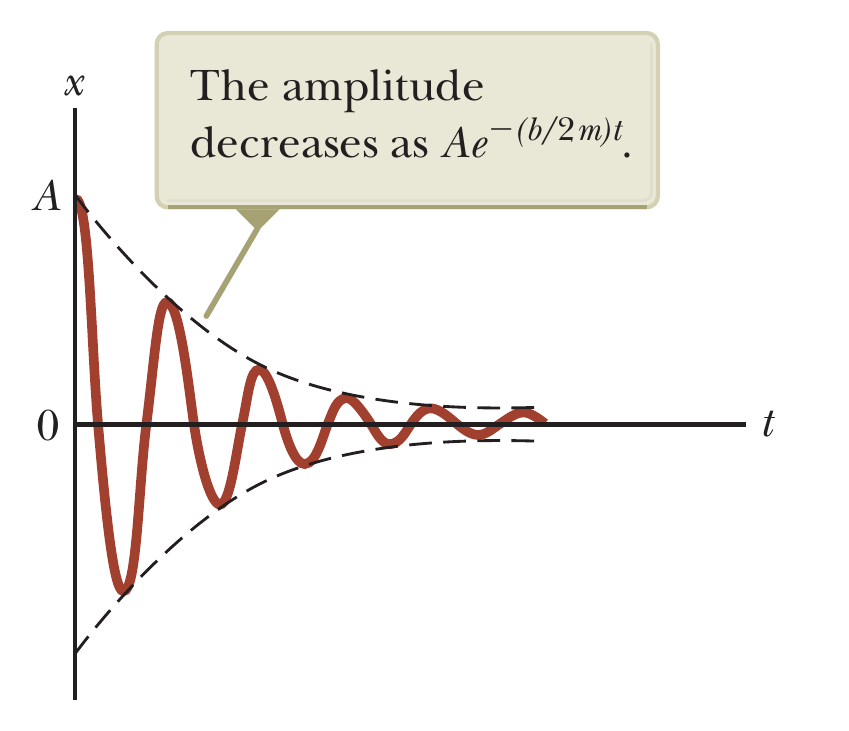
\includegraphics[scale=0.3]{images/oaw/damped01}
\end{center}

Consider the diagram above. Notice that with a small retarding force, the oscillating characteristic
of the motion is preserved but decreases exponentially. Eventually, that motion becomes undetectable.
Any system with this characteristic is known as a \textbf{damped oscillator}. The black dashed lines
are known as the \textbf{envelope} of the curve, showing the exponential decay of the amplitude.

Depending on the magnitude of the retarding force and $b$, it will have different effects on the
oscillation as shown in the following figure. Note that $\omega_0 = \sqrt{k/m}$ or the angular
frequency without the retarding force.
\begin{center}
    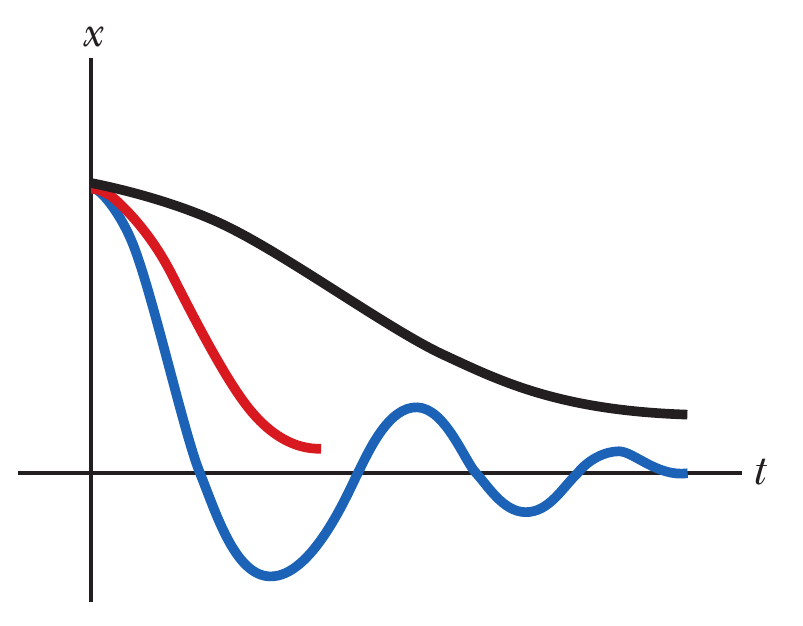
\includegraphics[scale=0.4]{images/oaw/damped02.png}
\end{center}
\begin{itemize}
    \item $b$ is small such that $b/2m < \omega_0$: the system is \textit{underdamped}, represented
        by the blue line
    \item $b$ reaches a critical point $b_c$ where $b_c/2m = \omega_0$: system does not 
        oscillate anymore and is said to be \textit{critically damped}, meaning once released from
        rest from some non-equilibrium position, it will approach, reach, but not pass the
        equilibrium point $-$ represented by the red line
    \item $b$ is large such that $b/2m > \omega_0$: the system is \textit{overdamped}, meaning it also
        does not oscillate and just returns to equilibrium position $-$ represented by the black line
\end{itemize}

Notice that as the damping increase, the interval taken for the system to approach equilibrium also increases.
In addition, there is no angular frequency in the case of the motion being critically damped or overdamped.
For a clearer picture, go to this \href{https://youtu.be/99ZE2RGwqSM}{link}.